% This is samplepaper.tex, a sample chapter demonstrating the
% LLNCS macro package for Springer Computer Science proceedings;
% Version 2.20 of 2017/10/04
%
\documentclass[runningheads]{llncs}
%


% inlined bib file
\usepackage{filecontents}

%\usepackage[compact]{titlesec}
%\usepackage{lipsum,mwe,cuted}
\usepackage{float}%%%%提供浮动体的[H]选项,进而取消浮动
\usepackage{caption}%%提供\captionof命令


\pagestyle{plain}


\usepackage{graphicx}
\usepackage{verbatim}
\usepackage{caption}
%

%\usepackage{algpseudocode}
%\usepackage{amsmath,amssymb,amsthm}

\usepackage{graphicx}
%\usepackage{geometry}
%\usepackage{subfigure}
\usepackage{url}
\usepackage{multirow}
\usepackage{listings}
\usepackage{cite}
\usepackage{array}
\usepackage{enumerate}
\usepackage{booktabs}
\usepackage{color}
\usepackage{soul}
\usepackage{multicol}
%\usepackage{algcompatible}
%\usepackage[compatible]{algpseudocode}

%\usepackage[algo2e]{algorithm2e}
%\usepackage{algorithm}
%\usepackage{algorithmic}
% Used for displaying a sample figure. If possible, figure files should
% be included in EPS format.
%
% If you use the hyperref package, please uncomment the following line
% to display URLs in blue roman font according to Springer's eBook style:
% \renewcommand\UrlFont{\color{blue}\rmfamily}

\begin{document}
%
\title{Contribution Title\thanks{Supported by organization x.}}
%
%\titlerunning{Abbreviated paper title}
% If the paper title is too long for the running head, you can set
% an abbreviated paper title here
%
\author{First Author\inst{1}\orcidID{0000-1111-2222-3333} \and
Second Author\inst{2,3}\orcidID{1111-2222-3333-4444} \and
Third Author\inst{3}\orcidID{2222--3333-4444-5555}}
%
\authorrunning{F. Author et al.}
% First names are abbreviated in the running head.
% If there are more than two authors, 'et al.' is used.
%
\institute{Princeton University, Princeton NJ 08544, USA \and
Springer Heidelberg, Tiergartenstr. 17, 69121 Heidelberg, Germany
\email{lncs@springer.com}\\
\url{http://www.springer.com/gp/computer-science/lncs} \and
ABC Institute, Rupert-Karls-University Heidelberg, Heidelberg, Germany\\
\email{\{abc,lncs\}@uni-heidelberg.de}}
%
\maketitle              % typeset the header of the contribution
%
\begin{abstract}
The abstract should briefly summarize the contents of the paper in
150--250 words.

\keywords{First keyword  \and Second keyword \and Another keyword.}
\end{abstract}
%
%
%


\section{Introduction}
\label{sec:intro}
Single sign-on (SSO) systems, such as OAuth, OpenID Connect (OIDC) and SAML, have been widely deployed for web authentication.
%nowadays as a convenient web authentication mechanism. 
SSO delegates user authentication on websites from online services (Relying Party, RP) to a third party (Identity Provider, IdP).
%, via a single authentication process. 
Using SSO, a user no longer needs to maintain multiple credentials for different RPs.
%, instead, she only maintains the credential for the IdP, which further provides identity proofs to RPs.
%For RPs, SSO shifts the burden of user authentication to IdPs and therefore reduces their security risks and costs. As a result, SSO has been widely integrated with modern web systems.
According to Alexa, the popular web traffic analysis site, 80 websites among the top-100 websites integrate SSO services~\cite{Alexa}.
%Meanwhile, many email and social networking providers such as Google, Facebook, Twitter, etc. have been actively serving as social identity providers to support social login.

However, the wide adoption of SSO also raises new privacy concerns. 
%Currently, more and more companies are interested in the users' online trace for business practices, such as accurate delivery advertising. For example, large internet service providers, such as Google, are interested in collecting users' online behavioral information for various purposes (e.g., Screenwise Meter~\cite{googlenews}). Now, by simply serving the IdP role, these companies can easily collect a large amount of data to reconstruct users' online traces. 
NIST~\cite{NIST2017draft} indicates that curious IdP or multiple collusive RPs could break the users' privacy in such ways. (1) \textbf{IdP-based login tracing}. The IdP knows the identities of the RP and user in each single login instance; (2) \textbf{RP-based identity linkage}. The RP learns a user's identity from the identity proof, so that malicious RPs could collude to link the user's login activities.
\begin{comment}
\item {\em IdP-based login tracing}. The IdP knows the identities of the RP and user in each single login instance.
%, to generate the identity proof.
%As a result, a curious IdP could discover all the RPs that the victim user attempts to visit and profile her online activities.
\item {\em RP-based identity linkage}. The RP learns a user's identity from the identity proof, so that malicious RPs could collude to link the user's login activities.
%When the IdP generates identity proofs for a user, while the same user identifier is used in identity proofs generated for different RPs, malicious RPs could collude to not only link the user's login activities at different RPs for online tracking but also associate her attributes across multiple RPs.
\end{comment}

%The IdP-based login tracing and RP-based identity linkage would bring the real threat to users. Imagine that, a user concerning her privacy would avoid leaving her full sensitive information at an application. She only leaves parts of her sensitive messages at each application, for example, using the real name on a social website and address on shopping website. And she would try not to leave any linkable message to avoid applications combining her information, such as email.
%However, the privacy leaks in SSO systems make her effort in vain. As long as a user employs the SSO system, such as Google Account, to log in to these applications, the applications providers and Google can combine her information based on the SSO account.


To protect user privacy, the Pairwise Pseudonymous Identifier (PPID) is suggested by NIST~\cite{NIST2017draft}, OIDC~\cite{OpenIDConnect} and SAML~\cite{SAMLIdentifier}.
%and popular SSO protocols, such as OpenID Connect (OIDC)~\cite{OpenIDConnect} and SAML~\cite{SAMLIdentifier}. 
That is, IdP should offer a user multiple individual IDs for different RPs. 
Thus, an RP cannot  correlate the  PPID  with user's PPID at another RP. 
%Thus, collusive RPs cannot link a user's logins targeting different RPs. 
More and more IdPs have adopted PPID to protect user privacy, such as Active Directory Federation Services and Oracle Access Management.
%~\cite{MS, Oracle}. 
And NORDIC APIS and CURITY also suggest adopting PPID in SSO to protect user privacy.
%~\cite{Nordic, Curity}.

Although PPID mechanism can protect user from RP-based identity linkage, the IdP-based identity linkage is not well prevented in SSO systems.
There have been many works on protecting user privacy in SSO systems, however, to the best of our knowledge, none of the existing techniques~\cite{SPRESSO, BrowserID, ZhangKSZR21, IsaakidisHD16} can offer the comprehensive protection of privacy or achieve it by integrating PPID. 
%Beside of PPID mechanism, there have been many works on protecting user privacy in SSO systems. 
Here we give a brief introduction of existing solutions
% for privacy-preserving SSO 
and explain the flaws of these schemes. 
\begin{itemize}
\item {\noindent\textbf{Simply hiding RP ID from IdP. }}For example, SPRESSO~\cite{SPRESSO} were proposed to defend against IdP-based login tracing by hiding RP ID from IdP. It uses the encrypted RP ID instead, and IdP issues the identity proof for this one-time encrypted ID. 
However, PPID is not available in this type of solution, as IdP cannot offer an RP a constant PPID with one-time irrelevant RP ID.
\item {\noindent\textbf{Proving user identity based on zero-knowledge proof. }}In this type of solution, such as EL PASSO~\cite{ZhangKSZR21}, the user needs to keep a secret $s$ and requires IdP to generate an identity proof for blinded $s$. Then user has to prove that she is the owner of $s$ without exposing $s$ to RP. 
However, whenever a user tries to visit RP at a new device, she must import  $s$ into this device. Thus, it is not convenient for user's login on multiple devices. 
%However, it is not convenient for user's login on multiple devices. For security consideration, the $s$ must be too long for user to remember.  And the user's identity is associated with the private $s$, therefore, if the user wants to log in to the RP on a new device, she must import the large $s$ into this device. 
%\item {\em Completely anonymous SSO system. }Anonymous SSO scheme is proposed to hide the user's identity to both the IdP and RPs in many manners. For example, the anonymous SSO~\cite{HanCSTW18} allows a user to visit the RP without exposing her identity to both IdP and RP based on zero-knowledge proof. However, it can only be applied to the anonymous services that do not identify the user, but not available in current personalized internet service.
\end{itemize}


%As discussed above, none of the existing SSO systems defend against both IdP-based login tracing and RP-based identity linkage, and provide the convenient SSO service on multiple devices at the same time.
%We remark that the problems cannot be solved, such as simply combining existing solutions together. The challenge is that, there is not a simple way for IdP to provide PPID without knowing the RP's identity.

In this paper, we propose UP-SSO, 
%Enhancing the User Privacy of SSO by Integrating PPID and SGX, 
the comprehensive protection against both IdP-based login tracing and RP-based identity linkage.
The key idea of UP-SSO is shifting PPID generation from server to user client,
so that IdP server can issue the identity proof containing user's PPID (denoted as $PPID_U$), by only requiring an one-time transformed RP ID (e.g., encrypted RP ID, denoted as $PPID_{RP}$). 
In UP-SSO system, the user client takes the responsibility for generating $PPID_U$ and transforming RP ID into $PPID_{RP}$,
%(as an identity proof must contain the RP ID to avoid misuse of token~\cite{YangLCZ18, WangZLG16, MainkaMS16, MainkaMSW17}). 
%For IdP, 
%it can only obtain an encrypted one-time RP ID, 
so that the IdP-based login tracing is not impossible as IdP no longer receives plain RP ID.
To be noticed is that the user-side service must be deployed at the user-controlled and IdP trusted environment, i.e., Intel SGX. 
With SGX, the secure hardware supported by intel CPU, the user-side service can be deployed at user's PC, and its integrity is guaranteed by \emph{Remote Attestation}, the mechanism provided by SGX.
%Moreover, other essential IdP services, such as user authentication and identity proof issuing,  must be deployed at server side for security consideration. 

%The overview of UP-SSO is shown in Figure~\ref{}. At the very beginning, user starts the visit to an RP (step 1). Then RP redirects user to IdP and the user is authenticated by IdP (step 2). After that, user invokes the user client (application protected by SGX) for PPID generation. To be noticed is that remote attestation must be conducted while the user client launches. After remote attestation, the user client and server are considered built a trust channel through a exchanged symmetric key. User client next retrieves the user ID (i.e., UID) from IdP server and RP (step 3). Then it generates the encrypted RP ID and PPID and sends them to IdP server to generate identity token (step 5). Following IdP issues the token with encrypted IDs and return it back to user ().   

%There have already been efforts on implementing authentication with security hardware, such as FIDO~\cite{fidouaf} UAF mode. It enables secure hardware (e.g., a smartphone) to store user's private key while the RP server stores the public key. Therefore, a user can be authenticated by the RP through a signed login challenge. However, compared with UP-SSO (as well as traditional SSO), FIDO does not provide an authority center, such as IdP. It brings about the problem that, the FIDO service cannot set accessibility limits without additional user information. For example, an RP requires that all the visitors must be adults. 
%In UP-SSO, the user only needs to be verified at IdP and the result can be included in an identity token. However, in FIDO system, the verification is not available except that user uploads specific information, which would link the user's accounts in different RPs. 

%To guarantee the security of UP-SSO, we provide the description of threat model and detailed systemic analysis, that shows UP-SSO prevents all the known attackers. Moreover, we have implemented a prototype of UP-SSO, including the servers, user client and user-side JavaScript codes. And we compare the performance of the UP-SSO prototype with a state-of-the-art SSO system (e.g., OpenID Connect). The time cost of UP-SSO and OpenID Connect is, respectively, about 154 and 113 ms. The overhead is modest.


\begin{comment}
We summarize our contributions as follows.
%我们的贡献
%提出协议
%考虑能否根据模型进行分析
%实现原型系统
%The main contributions of UPPRESSO are as follows:
\begin{itemize}
\item We propose the comprehensive solution to hide the users' login traces from both the curious IdP and malicious collusive RPs for convenient SSO system.
\item We formally analyze the security of XXX and show that it guarantees the security, while the users' login traces are well protected.
\item We have implemented a prototype of XXX, and compare the performance of the UP-SSO prototype with the state-of-the-art SSO systems (e.g., OIDC), and demonstrate its efficiency.
\end{itemize}
\end{comment}

\vspace{1mm}\noindent\textbf{Our contribution. }The main contribution of UP-SSO is that, it provides the PPID-included (containing $PPID_{RP}$ and $PPID_U$ ) identity proof without exposing RP ID to IdP, by shifting the $PPID_U$ generation from IdP server to user controlled device, and protecting it with the Intel SGX.
%we shift the PPID generation from IdP server to user controlled device, and protect it with the Intel SGX. It enables the IdP to provide the PPID-included identity token without exposing RP ID to IdP, while the user-side service is verified by IdP through remote attestation to guarantee its integrity.  
Therefore, UP-SSO offers the comprehensive solution to hide the users' login traces from both the curious IdP and malicious collusive RPs. 
%Moreover, it provides a new way of using secure hardware (i.e., Intel SGX) for SSO systems.

%文章结构
The rest of the paper is organized as follows. We first introduce the background in Section~\ref{sec:background}. Then, we describe the threat model, and our UP-SSO design in Sections~\ref{sec:threatmodel} and \ref{sec:design}, followed by a systemic analysis of security and privacy in Section~\ref{sec:analysis}. We provide the implementation specifics and experiment evaluation in Section~\ref{sec:implementation},  discuss the related work in Section~\ref{sec:relatedwork}, and conclude our work in Section~\ref{sec:conclusion}.

\section{Background}
\label{sec:background}
UP-SSO is compatible with OIDC, and achieves privacy protection based on the SGX.
Here, we provide a brief introduction on OIDC and the SGX.
\subsection{OpenID Connect and PPID}
OIDC~\cite{OpenIDConnect} is an extension of OAuth 2.0 to support user authentication, and has become one of the most prominent SSO authentication protocols. 
%Same as other SSO protocols~\cite{SAMLIdentifier}, OIDC involves three entities, i.e., {\em users}, the {\em identity provider (IdP)}, and {\em relying parties (RPs)}.
%PPID is suggested in OpenID Connect protocol to protect the user from a possible correlation among RPs.

\vspace{1mm}\noindent\textbf{Implicit flow of user login.}
OIDC supports three processes for the SSO authentication session, known as {\em implicit flow}, {\em authorization code flow} and {\em hybrid flow} (i.e., a mix-up of the previous two). Here, we choose the OIDC implicit flow as the example to illustrate the protocol. 
%In the implicit flow, an {\em id token} is generated as the identity proof, which contains a user identifier, an RP identifier, IdP's identifier, the validity period, and other requested attributes.
%The IdP signs the id token using its private key to ensure integrity.

\begin{figure}[t]
  \centering
  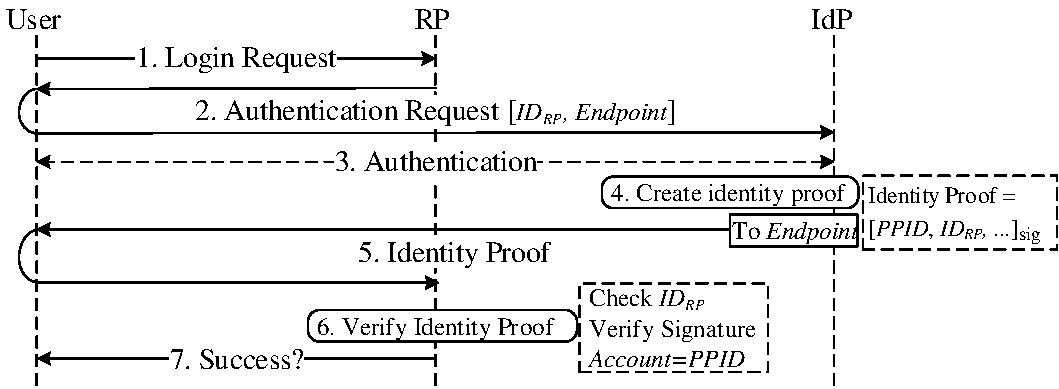
\includegraphics[width=\linewidth]{fig/OIDC1.pdf}
  \vspace{-5mm}
  \caption{The implicit protocol flow of OIDC.}
  \label{fig:OpenID}
  \vspace{-6mm}
\end{figure}

As shown in Figure~\ref{fig:OpenID}, 
At the beginning, user attempts to log in to an RP (step 1). Then RP constructs a request for identity proof, which is redirected by the user to the corresponding IdP. The request contains $ID_{RP}$, RP's endpoint other attributes (step 2). If the user has not been authenticated yet, the IdP performs an authentication process (step 3). Following, IdP signs the $ID_{RP}$ and PPID as the identity proof (step 4), and sends it back to the RP (step 5). Finally, the RP verifies the id token, extracts user identifier (step 6), and returns the authentication result to the user (step 7).
\begin{comment}
\item[1] At the beginning, user attempts to log in to an RP.
\item[2] RP constructs a request for identity proof, which is redirected by the user to the corresponding IdP. The request contains $ID_{RP}$, RP's endpoint other attributes.
\item[3] If the user has not been authenticated yet, the IdP performs an authentication process.
\item[4] IdP signs the $ID_{RP}$ and PPID as the identity proof.%If the RP's endpoint in the request matches the one registered at the IdP, it generates an identity token. Otherwise, IdP generates a warning to notify the user about potential identity proof leakage.
\item[5] IdP sends the identity proof back to the RP.
\item[6] The RP verifies the id token, and extracts user identifier.
\item[7] Finally, RP returns the authentication result to the user.
\end{comment}

\vspace{1mm}\noindent\textbf{Pairwise Pseudonymous Identifier (PPID).} 
PPID is the user identifier provided by IdP identifying a user. Different from the normal user ID, PPID is an RP-specific user ID. That is, while a user visits different RPs, IdP would provide different but constant user IDs (i.e., PPID) for these RPs.    
NIST~\cite{NIST2017draft} suggests that PPID should be either generated randomly and assigned to users by the IdP, or derived from other user's information if the derivation is done in an irreversible, unguessable manner. 
%that PPID should be used to prevent the user's account at the IdP from being easily linked at multiple RPs through use of a common identifier. 
%It also suggests that PPID should be either generated randomly and assigned to users by the IdP, or derived from other user's information if the derivation is done in an irreversible, unguessable manner (e.g., using a keyed hash function with a secret key). 
%For example, we have learned that, MITREid Connect, a popular open-source OIDC project, generates PPID using a secure random number generator, and stores the key-value map of corresponding RP and PPID.


\subsection{Intel SGX}
Intel Software Guard Extensions (Intel SGX)~\cite{costan2016intel} is the hardware-based security  mechanism provided by Intel processors.  Enclaves~\cite{costan2016intel} and remote attestation~\cite{costan2016intel} mechanism are offered by Intel SGX.
%It offers memory encryption that isolates specific application code and data in memory.
%It allows user-level code to allocate private regions of memory, called enclaves~\cite{costan2016intel}, which guarantees the running codes are well protected from the adversary outside the enclave.
 
\vspace{1mm}\noindent\textbf{Enclave.}
The enclave’s code and data is stored in Processor Reserved Memory (PRM). 
PRM cannot be directly accessed by other software, including system software and System Management Module code (Ring 2).
The Direct Memory Access (DMA) of PRM is also unavailable, as enclave is protected from other peripherals. That is, while the application is running inside the enclave, even the device owner cannot break its security, such as accessing or tempering the application's data.



\vspace{1mm}\noindent\textbf{Remote Attestation.} 
Remote attestation enables the software inside an  enclave to attest to a remote entity that it is trusted. 
%That is, during the attestation, the remote entity would receive an SGX attestation signature, containing the enclave’s measurement (a measurement of the code and data loaded in enclave).
The SGX remote attestation allows a player to verify the application's identity, intactness (never tampered), and that it is running securely within an enclave.
Moreover, with the remote attestation, the secure key exchange between the player and remote enclave application is also available.% even the application runs in a malicious environment.

 
\section{Threat Model}
\label{sec:threatmodel}
%UP-SSO is compatible with OIDC, consisted of a number of RPs, user agents(including browser and enclave application) and an IdP.
In this section, we describe the threat model and assumptions of the entities in UP-SSO.

\vspace{1mm}\noindent\textbf{Adversary Goal:} (1) The adversaries attempt to impersonate a user to log into an RP (\textbf{breaking the  security of SSO}); (2) the adversaries want to track a user's login trace (\textbf{breaking the privacy}).
\begin{comment}
\item \noindent\textbf{Breaking the security. }The adversaries can impersonate an honest user to log in to the honest RP.
\item \noindent\textbf{Breaking the privacy. }The adversaries can track a user's login trace on each RP.
\end{comment}

\vspace{1mm}\noindent\textbf{Adversary Capacity: }
\begin{itemize}
\item \noindent\textbf{To break the security.}
An adversary could act as a malicious user or a malicious RP.
The adversary could control the software running outside the enclave, capturing and tempering the message transmissions, decrypting and tempering the HTTPS flows, tempering the script code running on the browser.
Moreover, the attacker might also act as an external attacker,
    who collects all network traffics. The adversary could also allure the user to download the malicious script on his browser.

\item \noindent\textbf{To break the privacy.}
An adversary can act as the malicious RP and curious but honest IdP.
The malicious RP may manipulate  all the messages generated and transmitted by RP.
However, the honest IdP must process the requests of RP registration and identity proof correctly, provide honest script, and never collude with others.
Both RP and IdP can store and analyze the received messages.

%\item \noindent\textbf{An adversary can act as the malicious user.}
%An adversary can act as the malicious user.
%The adversary can control the software running outside the enclave, capturing and tempering the message transmission between enclave application and another entities, decrypting and tempering the HTTPS flows, tempering the script code running on the browser.
%For example, a malicious user may try to temper the PPID sent to IdP to achieve an identity token representing an honest user.
%\item \noindent\textbf{An adversary can act as the malicious RP. }
%An adversary can act as the malicious RP.
%The adversary can lead the user to log in to the malicious RP. In this situation, the adversary can manipulate  all the messages transmitted through RP, and collect all the flows received from user to link the user identity.
%\item \noindent\textbf{An adversary can act as the curious but honest IdP. }
%An adversary can act as the curious but honest IdP.
%The curious IdP can store and analyze the received messages.
%, and perform the timing attacks, attempting to achieve the IdP-based linkage.
%However, the honest IdP must process the requests of RP registration and identity proof correctly, provide honest script, and never collude with others.
%\item \noindent\textbf{External attackers. }An adversary can collect all the network flows. The adversary can also lead the user to download the malicious script on her browser.
\end{itemize}

%\subsection{Assumptions}
We assume the honest user's device is secure, for example, user would not install malicious application on his device.
The application and data inside the enclave are never tempered or leaked, even %in the malicious user's device.
the device is owned by an adversary.
Moreover, the enclave application always runs the processes same as IdP server expected, as it is guaranteed by remote attestation.

%The TLS is also adopted and correctly implemented in the system, so that the communications among entities ensure confidentiality and integrity.
%The cryptographic algorithms and building blocks used in UP-SSO are assumed to be secure and correctly implemented.

%Phishing attack is not considered in this paper.


\section{Design of UP-SSO}
\label{sec:design}
\begin{figure*}[t!]
  \centering
  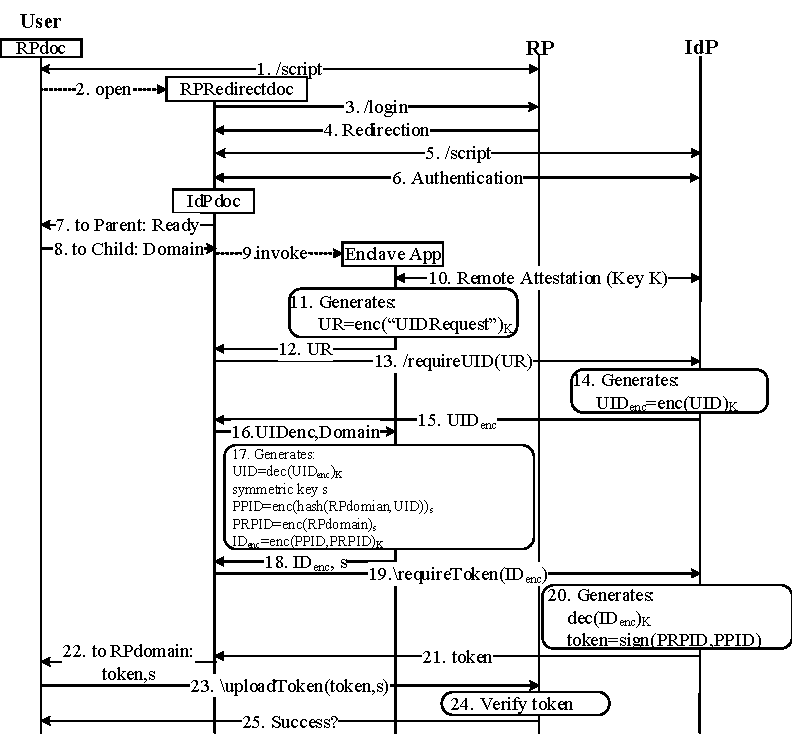
\includegraphics[width=0.8\linewidth]{fig/sgx-sso.pdf}
  \caption{The protocol flow of UP-SSO.}
  \vspace{-5mm}
  \label{fig:UP-SSO}
\end{figure*}
%The UP-SSO is compatible with OIDC, besides that the IdP service is separated into user part and server part. 
%The user agent (i.e., user-side IdP service) would obtain the UID from server part service, transform UID into the PPID, and encrypt the RPID and PPID with a one-time symmetric key to avoid IdP server digging out the RP's identity. As the enclave application is protected by SGX, it must not conduct any malicious behaviour. 
%The server-side IdP service takes the responsibility of authenticating the user, retrieving the UID for each user, and issuing the identity token (i.e., the identity proof) consisted the privacy-preserving RP and user identifier.

In this section, we will provide the detailed protocol.

%\subsection{UP-SSO procedures}
\subsection{Initialization}
%\vspace{1mm}\noindent\textbf{RP registration.} 
At the very beginning, RP needs to register its domain, RP name and other essential attributes at IdP, and obtains a signed Cert.  Thus, the  IdP can only provide the service to the qualified RP by checking the ownership of a Cert inside the enclave application.

%\vspace{1mm}\noindent\textbf{Preparation work of user .} 
Moreover, user should install the enclave application on her device before the visit targeting an RP. 

\subsection{Login Process}
Following, we provide the detailed process of each authentication flow shown as Figure~\ref{fig:UP-SSO}.
%The procedures of UP-SSO are depicted in detail in Figure~\ref{fig:UP-SSO}. 
It can be split into three phases, scripts downloading, PPIDs generation and identity proof issuing. To be noticed that, all the communication flows among user, RP server and IdP server are protected by TLS.

\vspace{0.5mm}\noindent\textbf{Scripts downloading.} This phase is for the user’s browser to download the scripts from the RP and IdP. The SSO process is started with the user's visit to an RP at her browser, and the browser downloads the RP script (step 1). Then the RP script opens a new window targeting RP login endpoint (step 2, 3). After that the user is redirected to the IdP server (step 4). Finally, the user retrieves the IdP script (step 5).

It must be noticed that, the user cannot visit IdP at step 2,3 directly. While the script in origin A opens a new window with origin B, the HTTP request to B's server will carry the key-value $Referer: A$ in the header. Thus, the RP's domain is exposed to IdP. 
% The scripts work as part of the user agent role.
\begin{comment}
\item[1]The SSO process is started with the user's visit to an RP at her browser, and the browser downloads the RP script. 
%The script is used to conduct the behaviour defined by RP on user side.
\item[2]The RP script opens a new window. 
\item[3]The newly opened window visits RP login endpoint.
\item[4]The user is redirected to the IdP server from RP.% login endpoint.
\item[5]The user retrieves the IdP script, which is used to deal with the interaction with other entities.% IdP server, RP script and enclave application.
\end{comment}
%It must be noticed that, the user cannot visit IdP at step 2,3 directly. While the script in origin A opens a new window with origin B, the HTTP request to B's server will carry the key-value $Referer: A$. Thus, the RP's domain is exposed.% to IdP. 
%With HTML5, a special attribute for links in HTML was introduced, that the $ref="noreferrer"$ can be used to make $Referer$ header be suppressed. However, when such a link is used to open a new window, the new window does not have a handle on the opening window (opener) anymore. The handle is necessary for UP-SSO to transmit messages between RP and IdP scripts. 
%So the redirection is adopted to avoid the HTTP header $Referer$. %and make the handle of the opening window available. 


\vspace{0.5mm}\noindent\textbf{PPIDs Generation.} In this phase, IdP script invokes the enclave application to generate the PPID. 
At first, the IdP authenticates the user (step 6). 
After that, IdP script informs RP window (step 7), and RP script sends its Cert to IdP script (step 8).  
Then IdP script asks for user's consent to visit targeting RP, and it invokes the enclave application (step 9). 
The enclave application conducts remote attestation at its initialized execution, and negotiates a symmetric key $K$ with IdP server (step 10).
Following the enclave application generates the UID request by encrypting request information with $K$ (step 11). 
The request is sent to IdP script (step 12) and transmitted to IdP server (step 13). 
IdP encrypts $UID$ with $K$ (step 14), and transmits it to enclave application through IdP script (step 15, 16).  
While receiving the encrypted $UID$, the enclave application derives the $UID$, verifies the Cert and achieves RP's domain from it, generates the symmetric key $S$, encrypts the RP's domain as the  $PPID_{RP}$, encrypts the hash of RP's domain and UID as the $PPID_U$, and encrypts $PPID_{RP}$ and $PPID_U$ with $K$ (step 17). 
Finally the encrypted IDs and $S$ are sent to IdP script (step 18). 

The $PPID_U$ must be the encrypted hash of RP's domain and UID, instead of the plain digest. It avoids the IdP to find out multiple logins targeting the same RP or not, as the hash of same RP's domain would be always the same. 

%Moreover, there are some types of parameters required in OIDC protocol to be carried in the SSO request, such as $response\_type$ and $scope$. In this paper, we would not mention these attributes, and only focus on the necessary parameters. 
\begin{comment}
\item[6]At first, the IdP authenticates the user.
\item[7]After the IdP script is downloaded, it sends the ready signal to its opener (i.e., the RP window).
\item[8]RP script sends the RP's Cert back to IdP script. 
\item[9] The IdP script shows RP name to user to make sure user would not visit malicious RP, and then it invokes the enclave application.
\item[10]The enclave application conducts remote attestation at its initialized execution. After the remote attestation, enclave application and IdP server share a symmetric key $K$.
\item[11]The enclave application generates the UID request (i.e., $UR$) by encrypting request information with $K$.
\item[12]$UR$ is sent to IdP script.
\item[13]Then the user starts the UID request to IdP.
\item[14]IdP encrypts $UID$ with $K$.
\item[15]IdP script receives encrypted $UID$ from IdP.
\item[16]IdP script transmits encrypted $UID$ and RP's domain to enclave application.
\item[17]The enclave application derives the $UID$ with $K$, verifies the Cert, achieves RP's domain from Cert, generates the symmetric key $s$, encrypts the RP's domain with key $s$ as the transformed RP ID (i.e., $PRPID$), encrypts the hash of RP's domain and UID as the $PPID$, and encrypts $PRPID$ and $PPID$ with $K$.
\item[18]Enclave application sends the encrypted IDs and $s$ to IdP script. 
\end{comment} 
%The PPID must be the encrypted hash of RP's domain and UID, instead of the plain digest. It avoids the IdP to find out multiple logins targeting the same RP or not, as the hash of same RP's domain would be always the same. 

%Moreover, there are some types of parameters required in OIDC protocol to be carried in the SSO request, such as $response\_type$ and $scope$. In this paper, we would not mention these attributes, and only focus on the necessary parameters. 

\vspace{0.5mm}\noindent\textbf{Identity proof issuing.} In this phase, IdP issues an identity proof containing the encrypted $PPID_{RP}$ and $PPID_U$. And the RP verifies the token.
At the beginning user sends the encrypted $PPID_{RP}$ and $PPID_U$ to IdP for identity proof (step 19). 
Then the IdP server derives the $PPID_{RP}$ and $PPID_U$, signs the $Token$ consisted of $PPID_{RP}$ and $PPID_U$ as the identity proof (step 20), and sends it to IdP script (step 21). 
The IdP script then sends the $oken$ and $s$ to the origin RP's $Domain$ through $postMessage$ (step 22), and  RP script uploads them to RP server (step 23). 
The RP server verifies the signature with IdP's public key, compares the $PPID_{RP}$ carried with identity proof with self-generated one, and derives the constant user account from $PPID_U$ (step 24). 
%generates the $PRPID$ with its domain and key $s$, and compared it with the one carried by $token$. If the two $PRPID$s are equaled, RP decrypts the user's account from $PPID$, and finds out the related user information in its database (step 24). 
At the end, RP returns the login result back to user (step 25).


\begin{comment}
\item[19]User sends the encrypted $PRPID$ and $PPID$ to IdP for identity proof.
\item[20]The IdP server derives the $PRPID$ and $PPID$, signs the $token$ consisted of $PRPID$ and $PPID$ as the identity proof.
\item[21]IdP sends identity token to enclave application.
\item[22]The IdP script then sends the $token$ and $s$ to the origin RP's $Domain$ through $postMessage$.
\item[23]The RP script uploads the $token$ and key $s$ to RP server.
\item[24]The RP server firstly verifies the signature with IdP's public key, then generates the $PRPID$ with its domain and key $s$, and compared it with the one carried by $token$. If the two $PRPID$s are equaled, RP decrypts the user's account from $PPID$, and finds out the related user information in its database.
\item[25]RP returns the login result back to user.
\end{comment} 

%The origin required in step 22 
%is essential for secure identity token transmitting.
%It 
%guarantees that only the script running in the RP window can receive the $Token$, that avoids the man-in-the-middle attack.


\end{document}
